\documentclass[../report.tex]{subfiles}

\begin{document}
\subsection{Tác tử - Agent}
Một tác tử phần mềm, hay gọi tắt là tác tử là một chương trình máy tính tồn tại trong một môi trường nhất định, 
tự động hành động phản ứng lại sự thay đổi của mội trường nhằm đáp ứng một mục tiêu đã được thiết kế trước. 
Thoả mãn các tính chất sau: 
\begin{itemize}
    \item Bền bỉ - Code không được thực thi theo yêu cầu mà chạy liên tục và tự động quyết định 
        khi nào nên thực hiện hành động nào. 
    \item Tự động - Có khả năng lựa chọn nhiệm vụ, sắp xếp mức độ ưu tiên, hành động hướng mục tiêu, 
        có khả năng tự quyết định mà không cần can thiệp từ con người. 
    \item Xã hội - Có khả năng hợp tác để thực hiện nhiệm vụ thông qua giao tiếp và phối hợp. 
    \item Phản ứng - Tác tử nhận thức từ môi trường và phản ứng lại nó một cách hợp lý. 
\end{itemize}

\subsubsection{Phân biệt tác tử với chương trình}
Tất cả tác tử là chương trình, nhưng chương trình có thể không là tác tử. Sự khác biệt đến từ các tính chất cơ bản của tác tử so với 
một chương trình bất kì. 

\subsubsection{Phân biệt tác tử với đối tượng}
\begin{itemize}
    \item Tác tử có tính tự động hơn là đối tượng.
    \item Tác tử có sự mềm dẻo trong hành vi, có sự phản ứng, tính xã hội. 
    \item Tác tử có thể có nhiều hơn một luồng xử lý. 
\end{itemize}

\subsubsection{Phân biệt tác tử với hệ chuyên gia}
\begin{itemize}
    \item Hệ chuyên gia không được gắn với môi trường. 
    \item Hệ chuyên gia không được thiết kế với khả năng phản xạ. 
    \item Hệ chuyên gia không xét đến tính xã hội của các vấn đề.
\end{itemize}

\subsection{Tác tử thông minh - Intelligent Agent}
Tác tử thông minh là một thực thể tự động, tiếp nhận thông tin từ môi trường và có khả năng tương tác lại môi trường 
và hướng hành động của nó nhằm đạt được một mục tiêu nào đó.
Tác tử thông minh có thể học và sử dụng kiến thức để đạt được mục tiêu. \cite{intelligent-agent-wiki}

\begin{figure}[H]
\centering
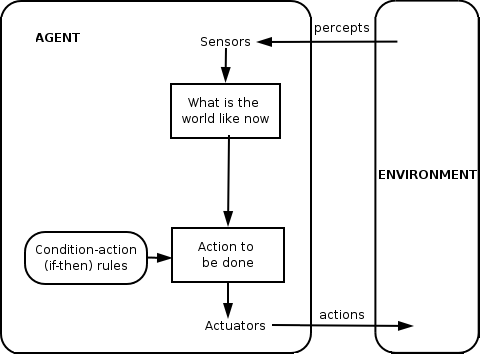
\includegraphics[width=10cm]{figures/simple-reflex-agent.png}
\caption{Simple reflex agent}
\end{figure}



\subsection{Hệ đa tác tử}
Hệ đa tác tử (multi-agent system) là một hệ tính toán được tạo thành bởi nhiều tác tử. \cite{multi-agent-system-wiki}


\end{document}
